\documentclass[11pt]{article}

\usepackage{fullpage}
\usepackage{enumitem}

\usepackage{amsmath,amsthm,amsfonts,amssymb,mathtools,latexsym}
\usepackage{xcolor,graphicx,hyperref,float}
\usepackage{tikz}
\usetikzlibrary{arrows.meta}

\usepackage[ruled,vlined,linesnumbered]{algorithm2e}

\pdfpagewidth 8.5in
\pdfpageheight 11in 

\oddsidemargin 0in
\evensidemargin 0in


\begin{document}
	
\begin{center}
\Large{\textbf{Homework 7}}
\end{center}

\section{Verifying Distances}
\subsection{a}
Designing a *linear time* algorithm that takes as input hte adjacency list $G$ as a nested hash table, source $s$, and hash table $dist$.
Return boolean expressions to verify that all distances in $dist$ are valid shortest path from $s$ to all other vertices after running Dijkstra's Algorithm.

\subsubsection{Pseudocode}
\begin{algorithm}[H]
    \small
    \caption{VerifyDijkstra($G$, $s$,$dist$)}
    \tcc{G: input adjacency list as a nested hash table}
    \tcc{s: source vertex}
    \tcc{dist: distances from source vertex $s$ to all other vertices(hash table)}

    \If{$dist[s] \ne 0$}{
        \tcc{if the source node's distance is not 0, invalid}
        return "incorrect"
    }

    \tcc{case 1: if $\pi(v) > d(u) + l(u,v)$}
    \tcc{we should maintain the invariant for all edges in $G$ for valid Dijkstra's output}
    \tcc{It is absolutely not valid if $\pi(v) > d(u) + l(u,v)$ for any edge because that means either there is a shorter path from $s$ to $v$ through $u$ or there exists a negative weight edge in the graph.}

    \For{u in G}{
        \For{v in G[u]}{
            $weight \gets G[u][v]$
            \If{$dist[v] > dist[u] + weight$}{
                return "incorrect"
            }
        }
    }

    \tcc{case 2: after setting up upper bound for the candidates, we only need the ones that strictly satisfy the invariant from the class regarding the valid distance of each node}
    \tcc{First, run BFS on $G$ so that we check every node in $G$, just like Dijkstra's algorithm does for shortest path by visiting every node in the graph.}
    $opt_cand \gets \text{empty hash table}$
    $Q \gets \text{empty queue}$ \tcc{this is not a Priority Queue so there is no $extract_min()$ and $decrease_key()$ operations that would require additional logrithmic runtime.}
    $Q.enqueue(s)$
    $opt_cand.add(s)$
    \While{!Q.isEmpty()}{
        $u \gets Q.dequeue()$

        \For{v in G[u]}{
            $weight \gets G[u][v]$
            \tcc{we only add the ones that are valid by the invariant: pi(v) = d(u) + l(u,v)}
            \If{$dist[u] = dist[v] + weight$}{
            \If{$v \notin \mathrm{opt\_cand}$}{
                    $\mathrm{opt\_cand}.add(v)$
                    $Q.enqueue(v)$
                }
            }
        }
    }

    \tcc{now we check if the possible valid candidate hash table is correct}
    \tcc{1. if the node is in the candidate hash table (or we included that node as one of the shortest pathways in BFS), then its weight should not be infinity because we recorded the constant weight}
    \tcc{2. otherwise, the weight should be infinity because we do not go through that node for shortest path.}
\For{v in G}{
        \If{$v \in \mathrm{opt\_cand}$}{
            \If{$dist[v] = \infty$}{
                return "incorrect"
            }
        }
        \Else{
            \If{$dist[v] \ne \infty$}{
                return "incorrect"
            }
        }
    }
    return "correct"
\end{algorithm}    

\subsubsection{Runtime Analysis}
\begin{enumerate}[label=\arabic*.]
    \item $O(1)$: constant time to check if source node is correct
    \item $O(n+m)$: linear time to set the upper bound for all nodes in the graph ($\pi(v) > min_{u \in S, v \in adj(u)} d(u) + l(u,v)$)
    \item $O(n+m)$: linear time to run BFS to create possible candidate distance hash table that Dijkstra's algorithm would have created.
    \item $O(n)$: linear time to compare the input distance table with possible candidate distance table to see if there exsits any node missing or overcounted.
\end{enumerate}
Therefore, the total runtime of the algorithm above is $O(1) + O(n+m) + O(n+m) + O(n) = O(n+m)$.

\subsubsection{Proof of Correctness}
For Dijkstra's algorithm to be correct:
\begin{enumerate}
\item $\pi(v) = min_{u \in S, v \in adj(u)} d(u) + l(u,v)$
\item If $u \in S$, then $d(u) = \delta(s,u)$
\item Every vertex in $G$ does not have weights of $\infty$ if it is reachable from the source vertex $s$.
\end{enumerate}

The algorithm checks if those three claims hold for the distance hash table $dist$.

\begin{enumerate}
\item The first claim is checked in the first case ($\pi(v) > min_{u \in S, v \in adj(u)} d(u) + l(u,v)$) in the algorithm to restrict upper bound of $\pi(v)$ for each node in $G$ to $\pi(v) = min_{u \in S, v \in adj(u)} d(u) + l(u,v)$.
\item Then, with the BFS implementation to iterate through $G$ to verify the equality.
\item Lastly, to check if every node on the shortest path is accounted, we run the last for loop to check if the node is in the candidate hash table and the node's weight is not $\infty$ or vise versa. 
\end{enumerate}

Therefore, the algorithm always verify the distance produced by Dijkstra's algorithm that $dist$ is the shortest path.

\subsection{(b) Parent Reconstruction Algorithm}
\subsubsection{Pseudocode}
\begin{algorithm}[H]
    \small
    \caption{reconstruct($G$, $s$,$dist$)}
    \tcc{G: input adjacency list as a nested hash table}
    \tcc{s: source vertex}
    \tcc{dist: distances from source vertex $s$ to all other vertices(hash table)}
    \tcc{the maximum length of the parent hash table is the number of vertices; space: O(n)}
    $parents \gets \text{hash table with n null values filled}$ \tcc{$n = |V|$}

    \tcc{loop through the adjacency table to find parents of each node that goes through shortest path}
    \tcc{dijkstra's algorithm determines the shortest path with greedy approach that selects a node of a distance that equals the sum of minimum total distance of previous node that directs to current node and the weight}
    \For{u in G}{
        \For{v in G[u]}{ 
            $weight \gets G[u][v]$ \tcc{weight extraction from $G$}
            \tcc{Three conditions to check}
            \tcc{1. make sure it is not a source node; it is root such that it cannot have a parent}
            \tcc{2. make sure we visited that node so dist[u] cannot be $\infty$}
            \tcc{3. distance of current node must be equal to the sum of minimum distance of previous node and its weights}
            \If{v != s $\cap$ dist[u] != $\infty$ $\cap$ dist[v] == dist[u] + weight}{
                $parents[v] \gets u$ \tcc{update parent if passed the conditions}
            }
        }
    }
    return $parent$
\end{algorithm}

\subsubsection{Runtime Analysis}
\begin{itemize}
\item $O(n)$: `parents` hash table initialization. Because we have to initialize it with at most length $n$, we need to iterate through $n$ times to assign `null` value to each index of `parents`
\item $O(n+m)$: we have to iterate through $G$ adjacency graph to check the conditions given above. while condition check only takes constant time $O(1)$, we need to check for every vertex to find the parent nodes through the shortest path possible.
\end{itemize}

Therefore, the total runtime of the algorithm is $O(n) + O(n+m) = O(n+m)$.

\subsubsection{Proof of Correctness}
To reconstruct `parents` hash table, a table that contains the parent of each node that goes through the shortest path, 
\begin{itemize}
\item we have to make sure if `dist` given is valid
\item we have to make sure if the parent of the source node does not exist
\item we have to make sure if all nodes in `parents` were visited  
\item we have to make sure if the distance of child node must equal to the sum of the minimum distance of parent node and the edge weight between the child and its parent nodes. 
\end{itemize}

Because the algorithm assumes that the output of (a) is "correct", `dist` must always be valid and contains the shortest path from the source to every node in $G$.
Also, 2,3, and 4 are checked at if condition inside the for loop that iterates through the adjacency list $G$.

Therefore, the algorithm above always reconstructs `parents` hash table that has every edge between nodes through the shortest path correctly.

\subsection{c}
\begin{center}
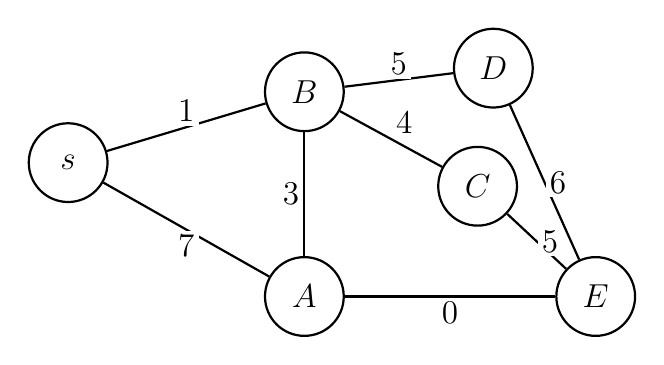
\begin{tikzpicture}[
    >=Stealth,
    vertex/.style={circle,draw=black,thick,minimum size=10mm,inner sep=1pt,font=\large},
    edge/.style={thick},
    weight/.style={fill=white,inner sep=1.5pt,font=\large}
]
    % Vertices
    \node[vertex] (S) at (0,1.8) {$s$};
    \node[vertex] (B) at (3.0,2.7) {$B$};
    \node[vertex] (A) at (3.0,0.1) {$A$};
    \node[vertex] (C) at (5.2,1.5) {$C$};
    \node[vertex] (D) at (5.4,3.0) {$D$};
    \node[vertex] (E) at (6.7,0.1) {$E$};

    % Weighted undirected edges
    \draw[edge] (S) -- node[weight,above] {1} (B);
    \draw[edge] (S) -- node[weight,below] {7} (A);
    \draw[edge] (B) -- node[weight,left] {3} (A);
    \draw[edge] (B) -- node[weight,above right] {4} (C);
    \draw[edge] (B) -- node[weight,above] {5} (D);
    \draw[edge] (C) -- node[weight,right] {5} (E);
    \draw[edge] (D) -- node[weight,right] {6} (E);
    \draw[edge] (A) -- node[weight,below] {0} (E);
\end{tikzpicture}
\end{center}
\end{document}
